\section{Evaluation}
We evaluate \myds and Phoenix on 
a 32-core Intel 4× Xeon E7-4820 system equipped with 128GB of RAM. 
The operating system is Ubuntu 12.04 with kernel 3.2.0 and glibc-2.15.
Benchmarks were built as 64-bit executables with gcc -O3.
We logically disable CPU cores using Linux’s CPU hotplug mechanism, 
which allows to disable or enable individual CPU cores 
by writing “0” (or “1”) to 
a special pseudo file (/sys/devices/system/cpu/cpuN/online), 
and the total number of threads was matched to the number of CPU cores enabled.
Each workload is executed 10 times. 
To reduce the effect of outliers, 
the lowest and the highest runtimes for each workload are discarded, 
and thus each result is the average of the remaining 8 runs.

\subsection{Performance of benchmarks}

\begin{figure}[htpb]
\centering
  \subfigure[]{
   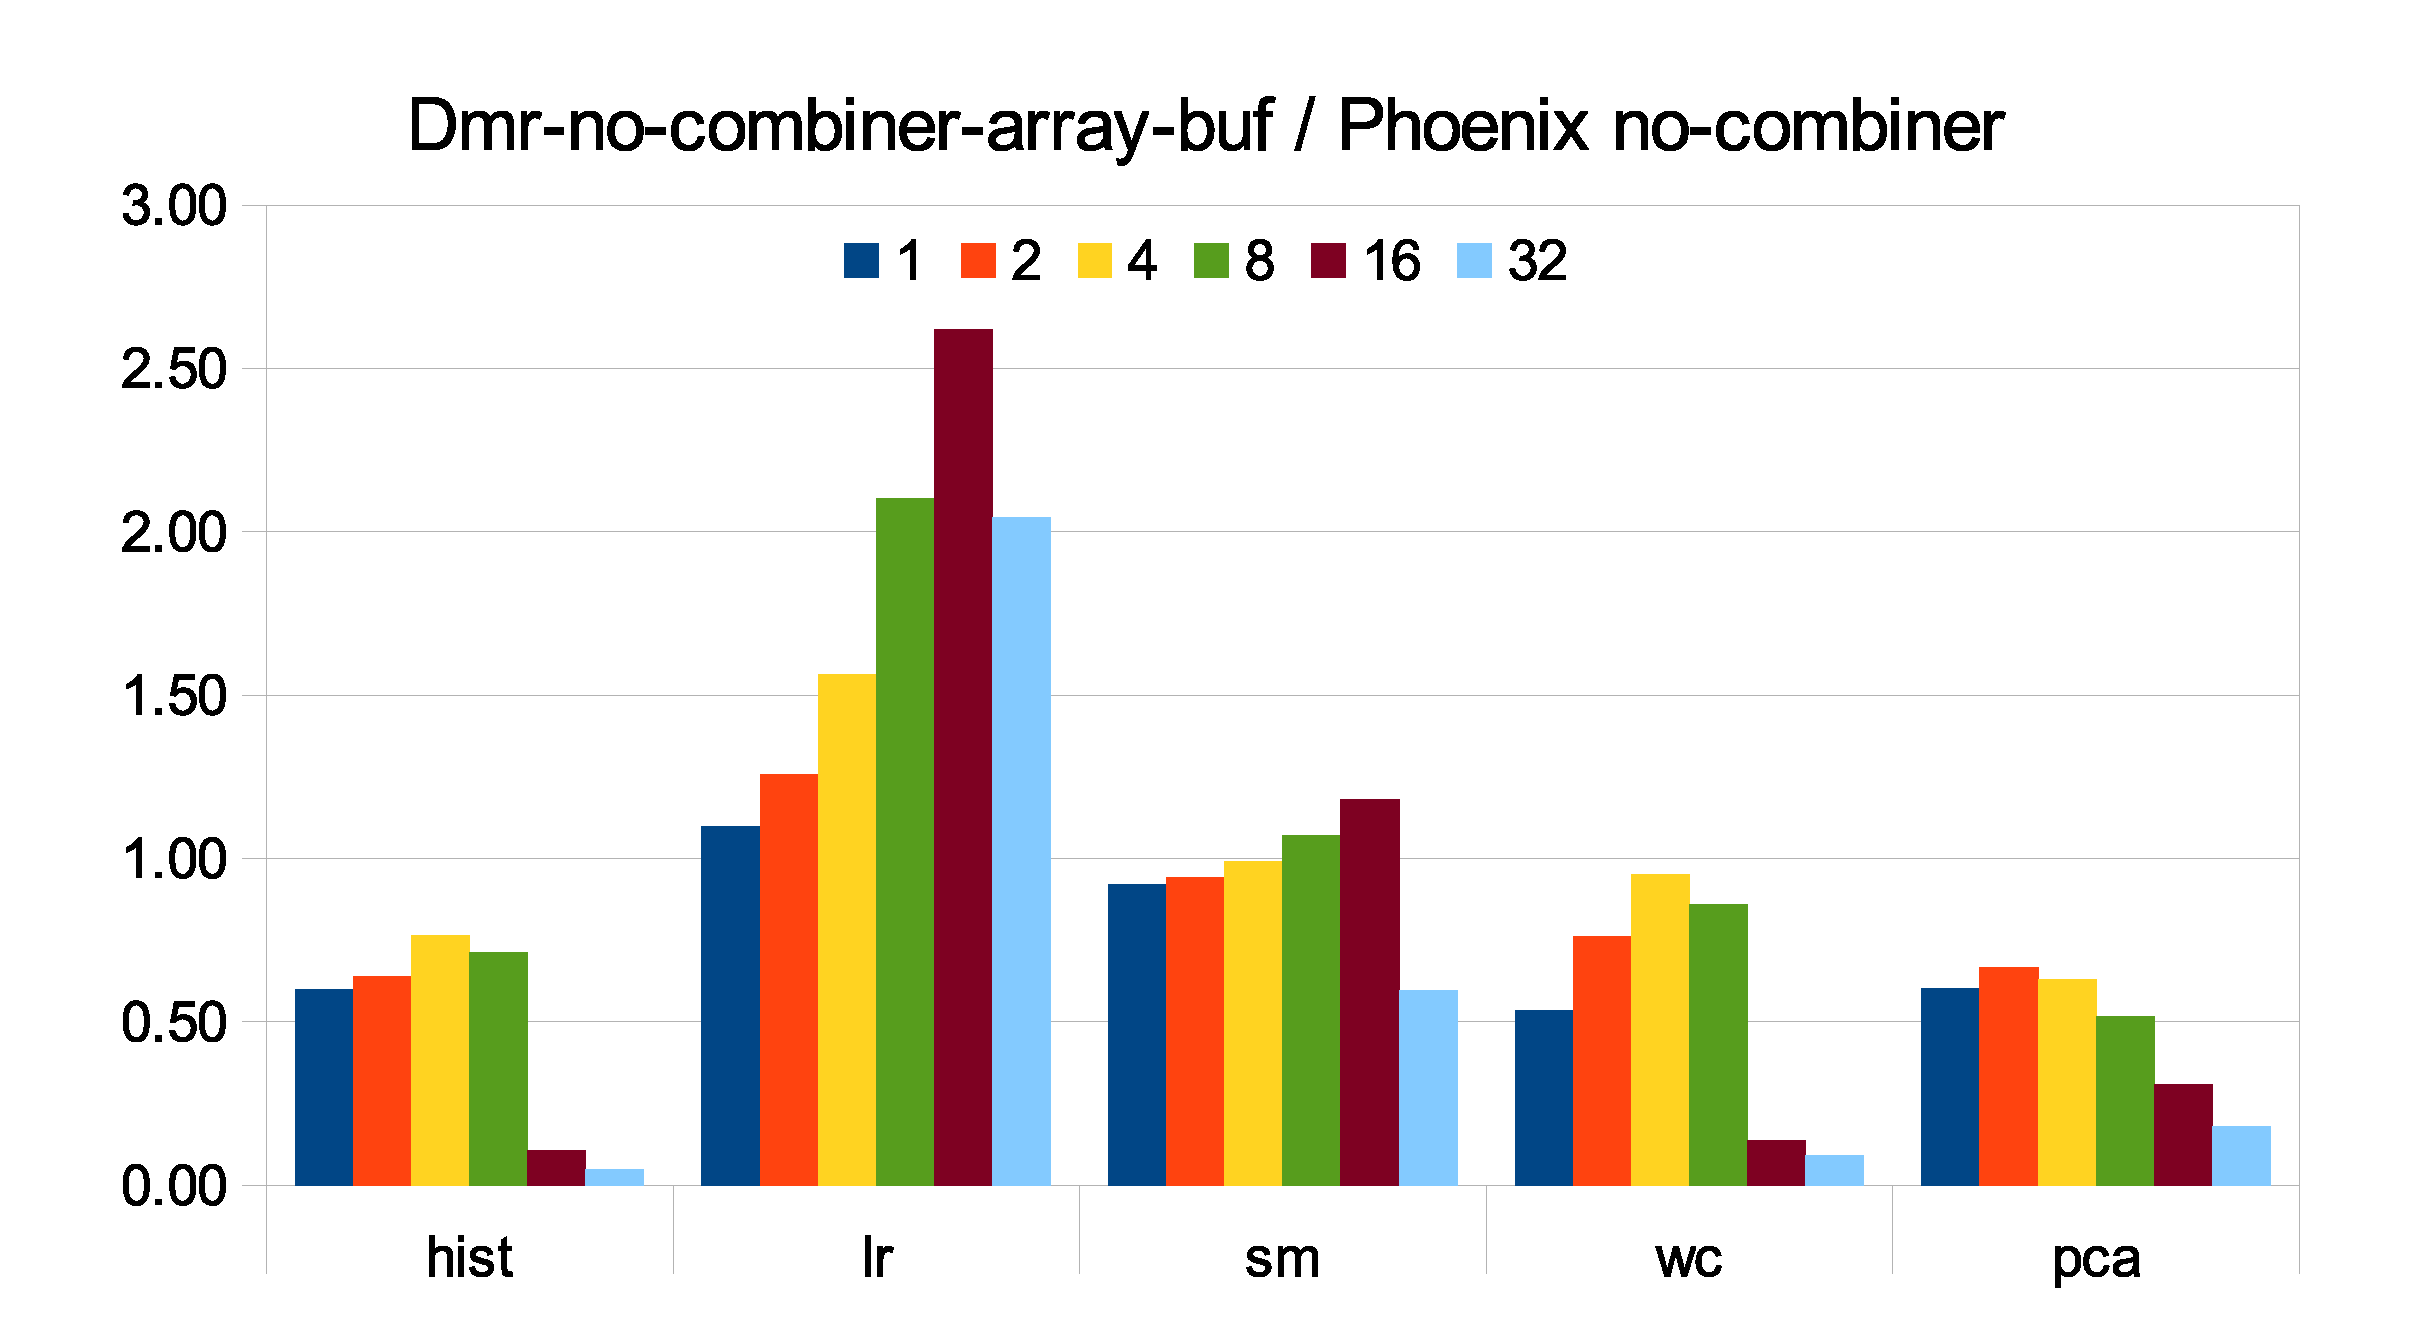
\includegraphics[width=0.4\textwidth]{eps/dmr_time_array.eps}
   \label{fig:dmr:time:ptmalloc}
  }
  \subfigure[]{
   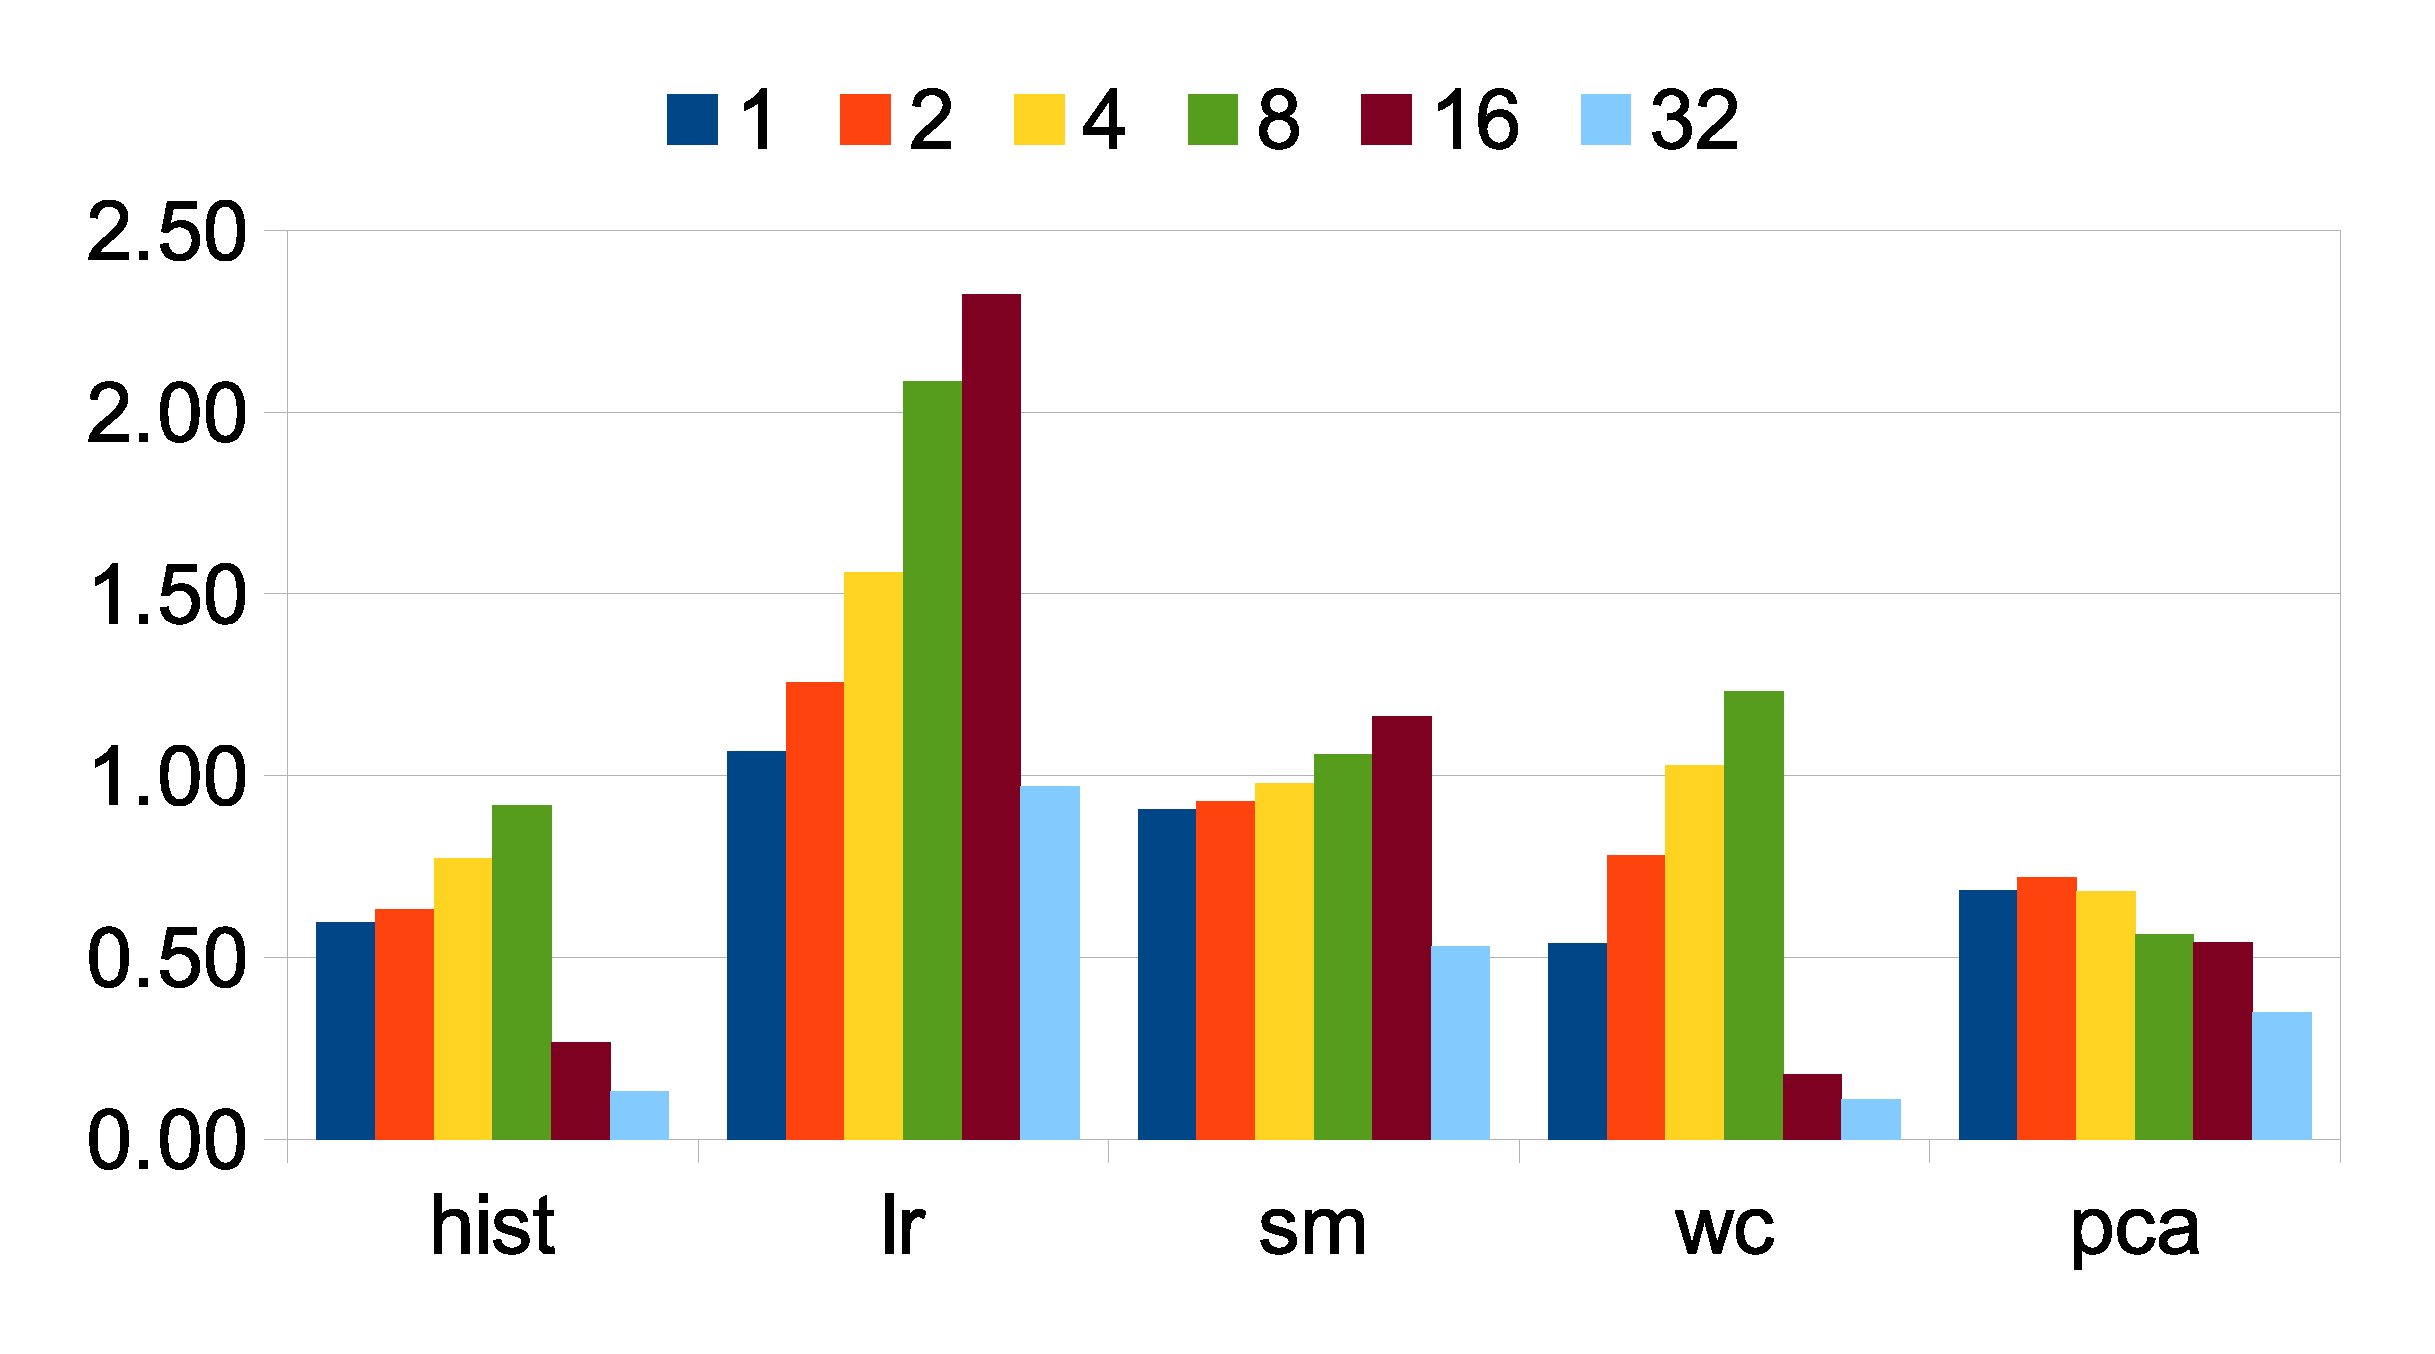
\includegraphics[width=0.4\textwidth]{eps/dmr_time_jemalloc.eps}
   \label{fig:dmr:time:jemalloc}
  }
  \caption{Execution time of SMR versus Phoenix}
   \label{fig:time}
\end{figure}

{\bf Performance}
We compare \myds with Phoenix, built with different memory allocator: ptmalloc and jemalloc.
Since there are many heap objects shared among threads
in Phoenix, and ptmalloc\cite{gloger1997ptmalloc}, 
the memory allocator in glibc, does not scale on multicore system. 
Then we evaluation Phoenix built with jemalloc\cite{evans2006jemalloc}, 
a scalable memory allocator for multicore system.

Figure\ref{fig:dmr:time:ptmalloc} and \ref{fig:dmr:time:jemalloc}
present the Execution time of \myds versus Phoenix.
%虽然jemalloc的性能表现要比ptmalloc好,但实验结果都显示
\myds matches or outperforms Phoenix on 4 out of 5 workloads,
but runs worse than Phoenix only on linear\_regression.
For hist, pca and word\_count, 
\myds outperforms Phoenix betwen xxx and xxx faster.
The reason of worse performance on linear\_regression 
is that most of time is waste in \myds's initailization.
We will evaluation overhead of initialization time in section\ref{}.
%从实验的结果可以看出,hist, wc, pca,SMR的性能较好,sm相当,lr中SMR的性能表现较差



\begin{figure}[htpb]
\centering
  \subfigure[]{
   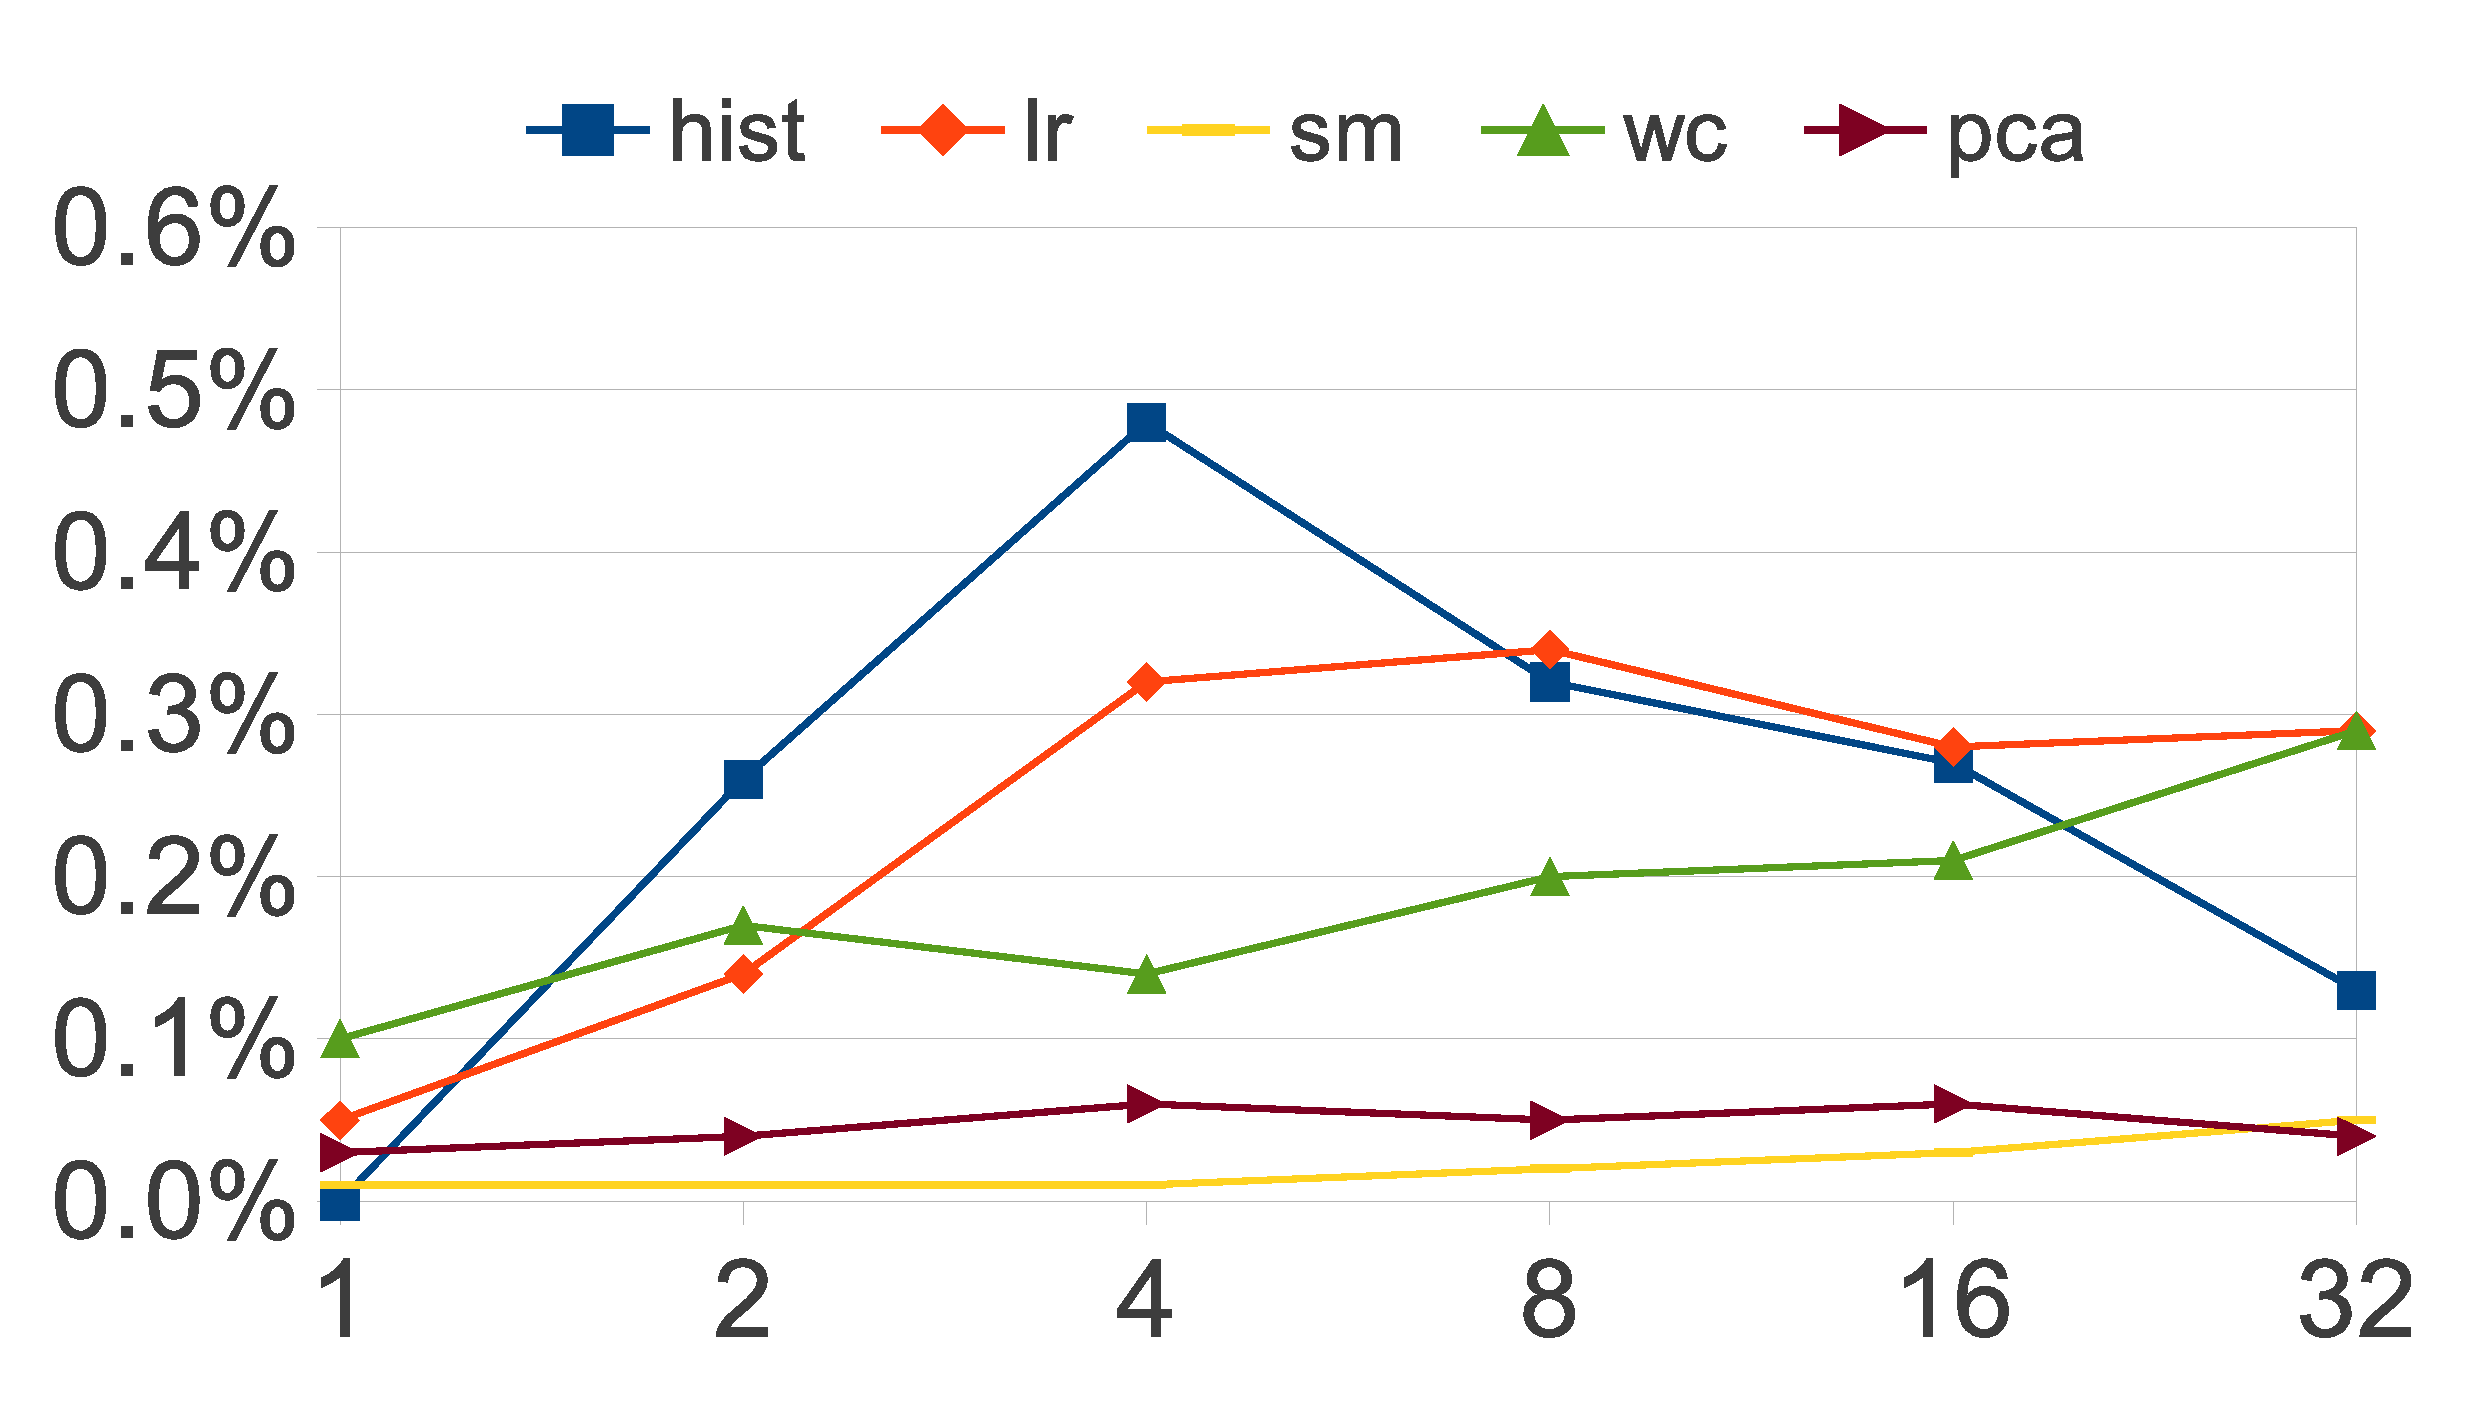
\includegraphics[width=0.25\textwidth]{eps/dmr_spinlock.eps}
   \label{fig:dmr:time:ptmalloc}
   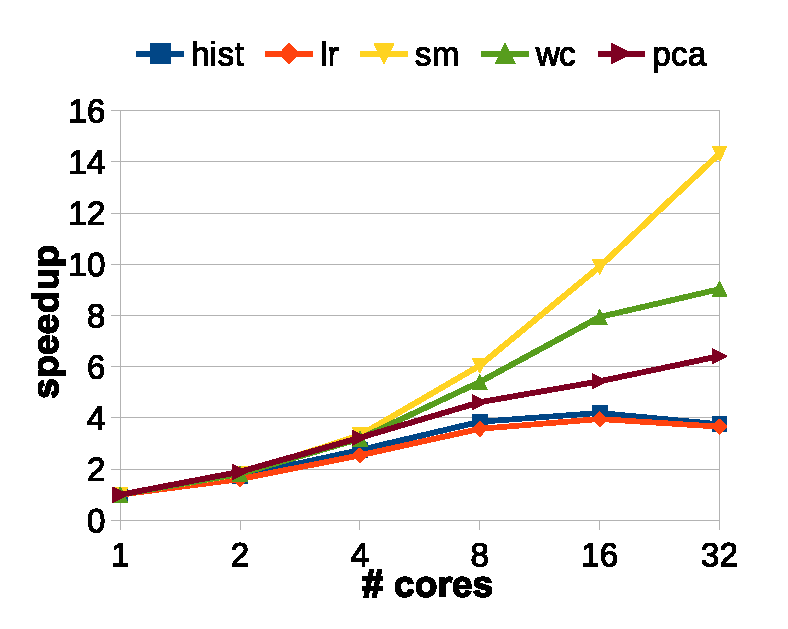
\includegraphics[width=0.25\textwidth]{eps/dmr_speedup.eps}
   \label{fig:dmr:time:jemalloc}
  }
  \caption{Scalability of SMR}
   \label{fig:scalability}
\end{figure}
{\bf Scalability}


We say a waiting thread is the thread which is waiting for shared
data that produced by another thread. If using semaphore for
synchronization, a waiting thread will be blocked and enlisted
on the waiting queue by the OS scheduler. If using spinlock
for synchronization, a waiting thread will do busy wait, i.e.
spinning in a while loop. Embedded software applications
that using semaphore to handle the synchronization could
result in performa+nce overkill, since it involves system calls
translated into thousands of CPU instructions [1]; while using
spinlock have problem of long busy-waiting time.

When a running thread tries to read shared data,
it must do busy wait until it has exhausted its time-slice
or until another thread has withdrawn the occupation on the
shared data. 




System performance is evaluated using
instructions per cycle (IPC). Higher IPC means
better performance.
Figure \ref{fig:perf:ipc} shows the IPC of Phoenix first increases 
and then decreases as more threads are run on multi-core system.


{\color{red}\myds }
Evaluation indicates that
the locking overhead can be significantly reduced to less
than 1% of total runtime on 32 cores




%分析lr性能差的原因

The performance of hist, wc, sm are scale linearly with the number of cores.


\subsection{Overhead of SMR}
\begin{figure}[htpb]
\centering
  \subfigure[]{
   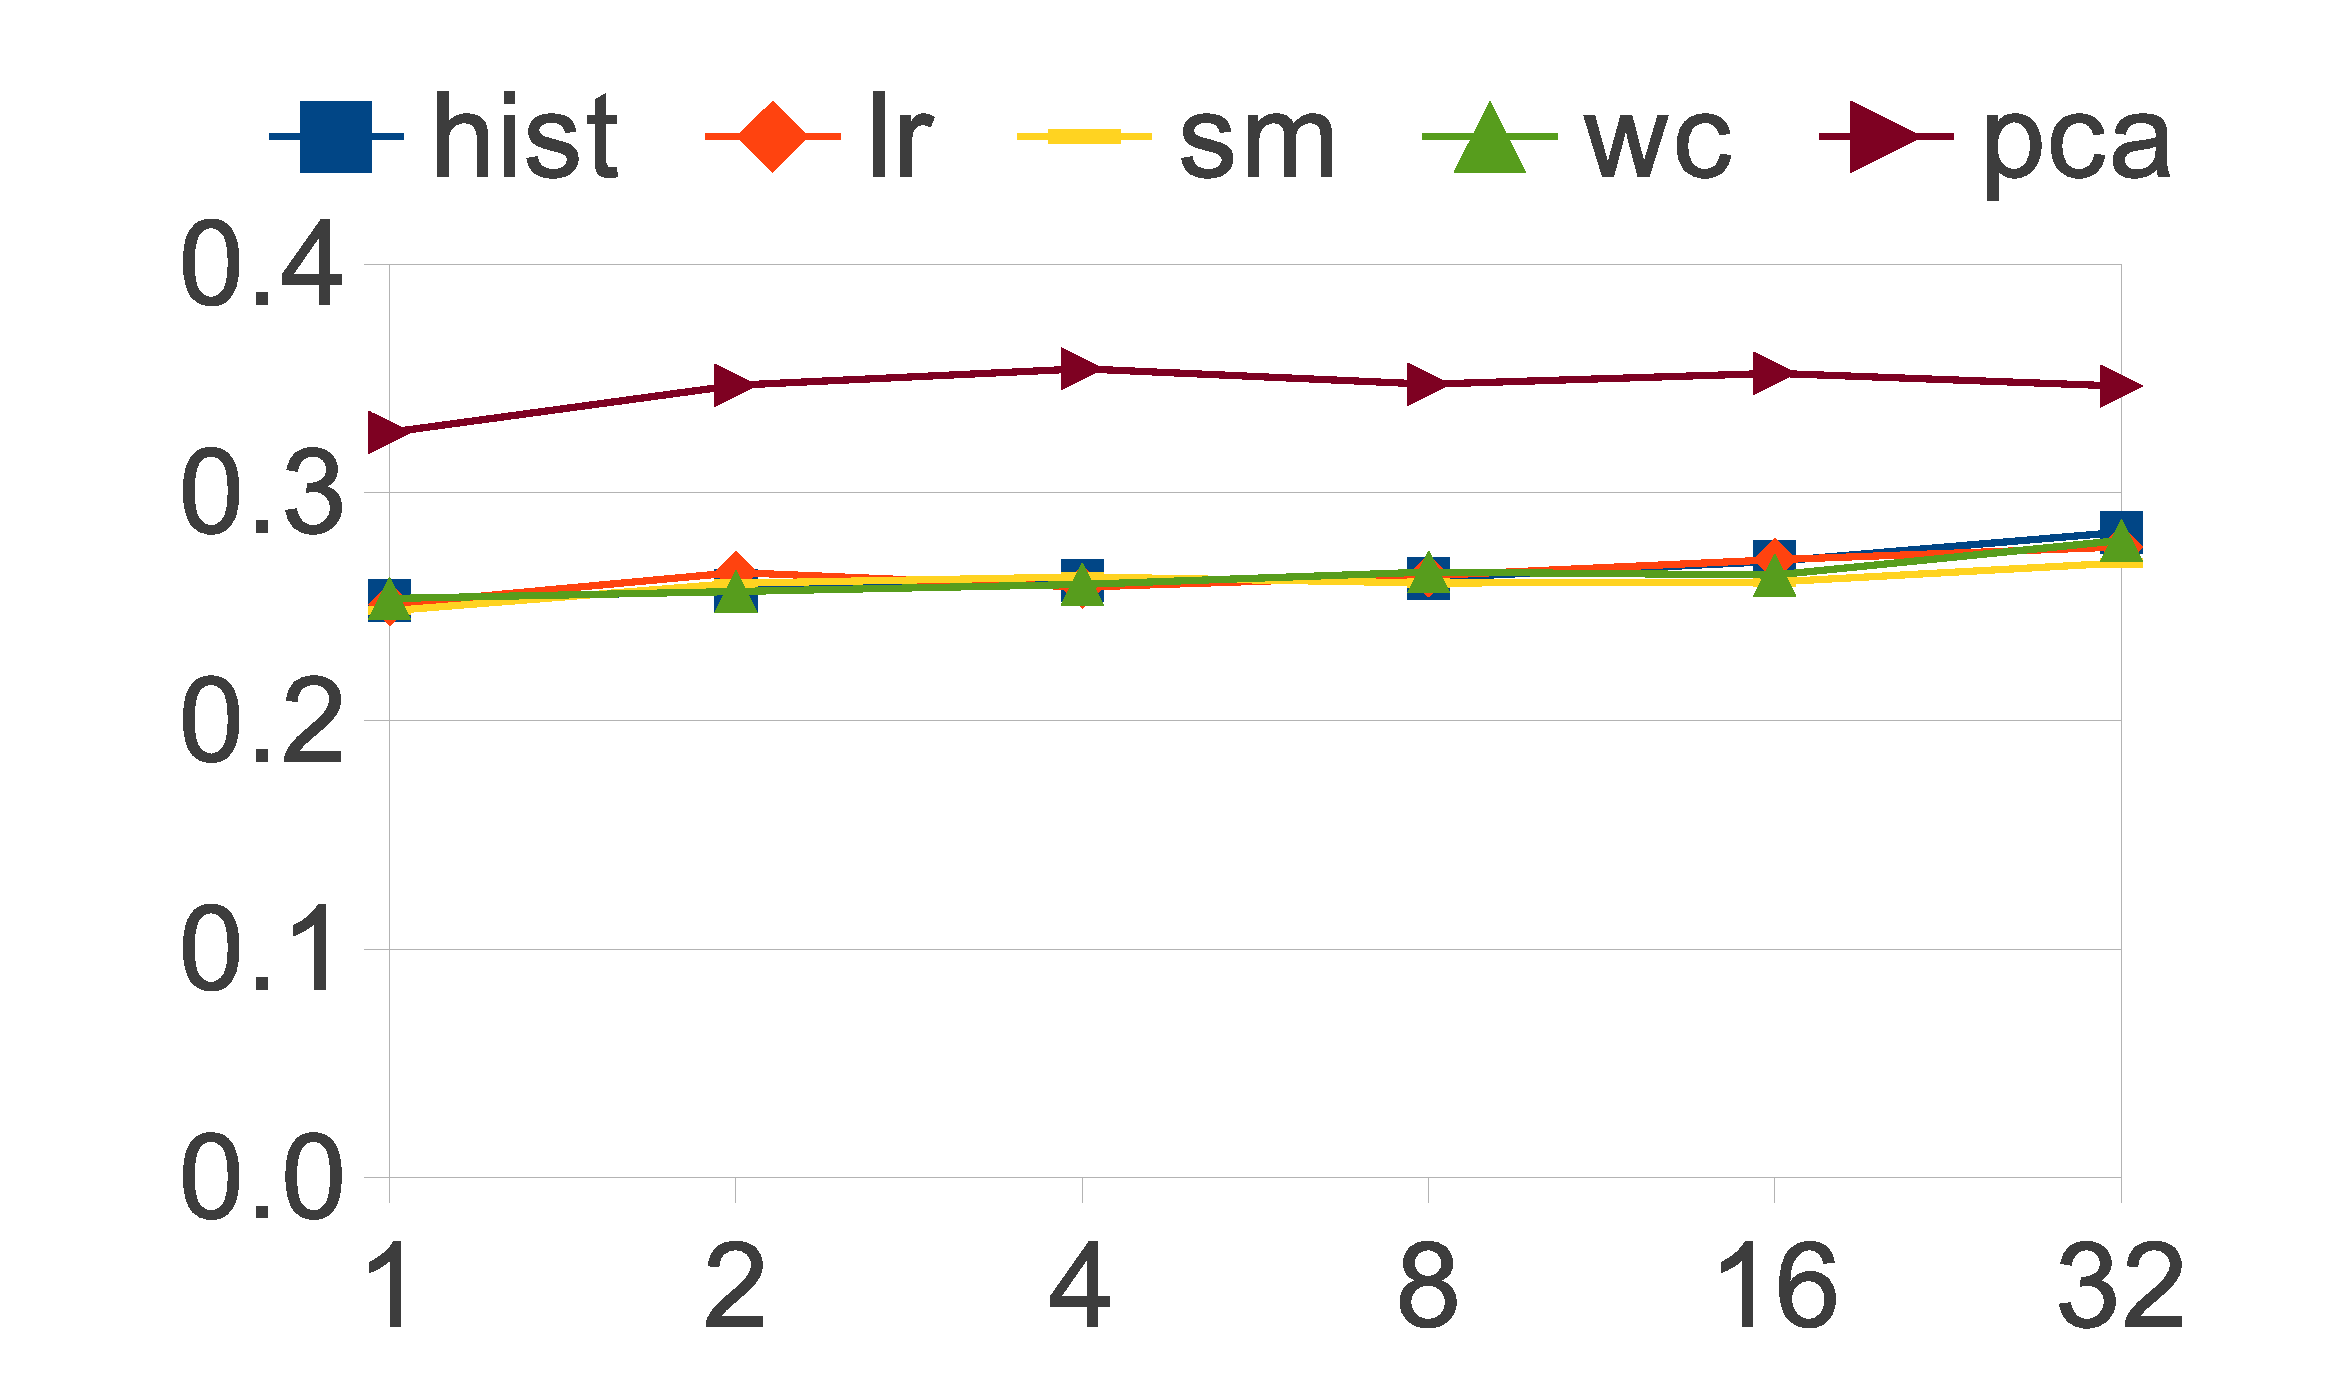
\includegraphics[width=0.25\textwidth]{eps/dmr_init_time.eps}
   \label{fig:dmr:time:ptmalloc}
   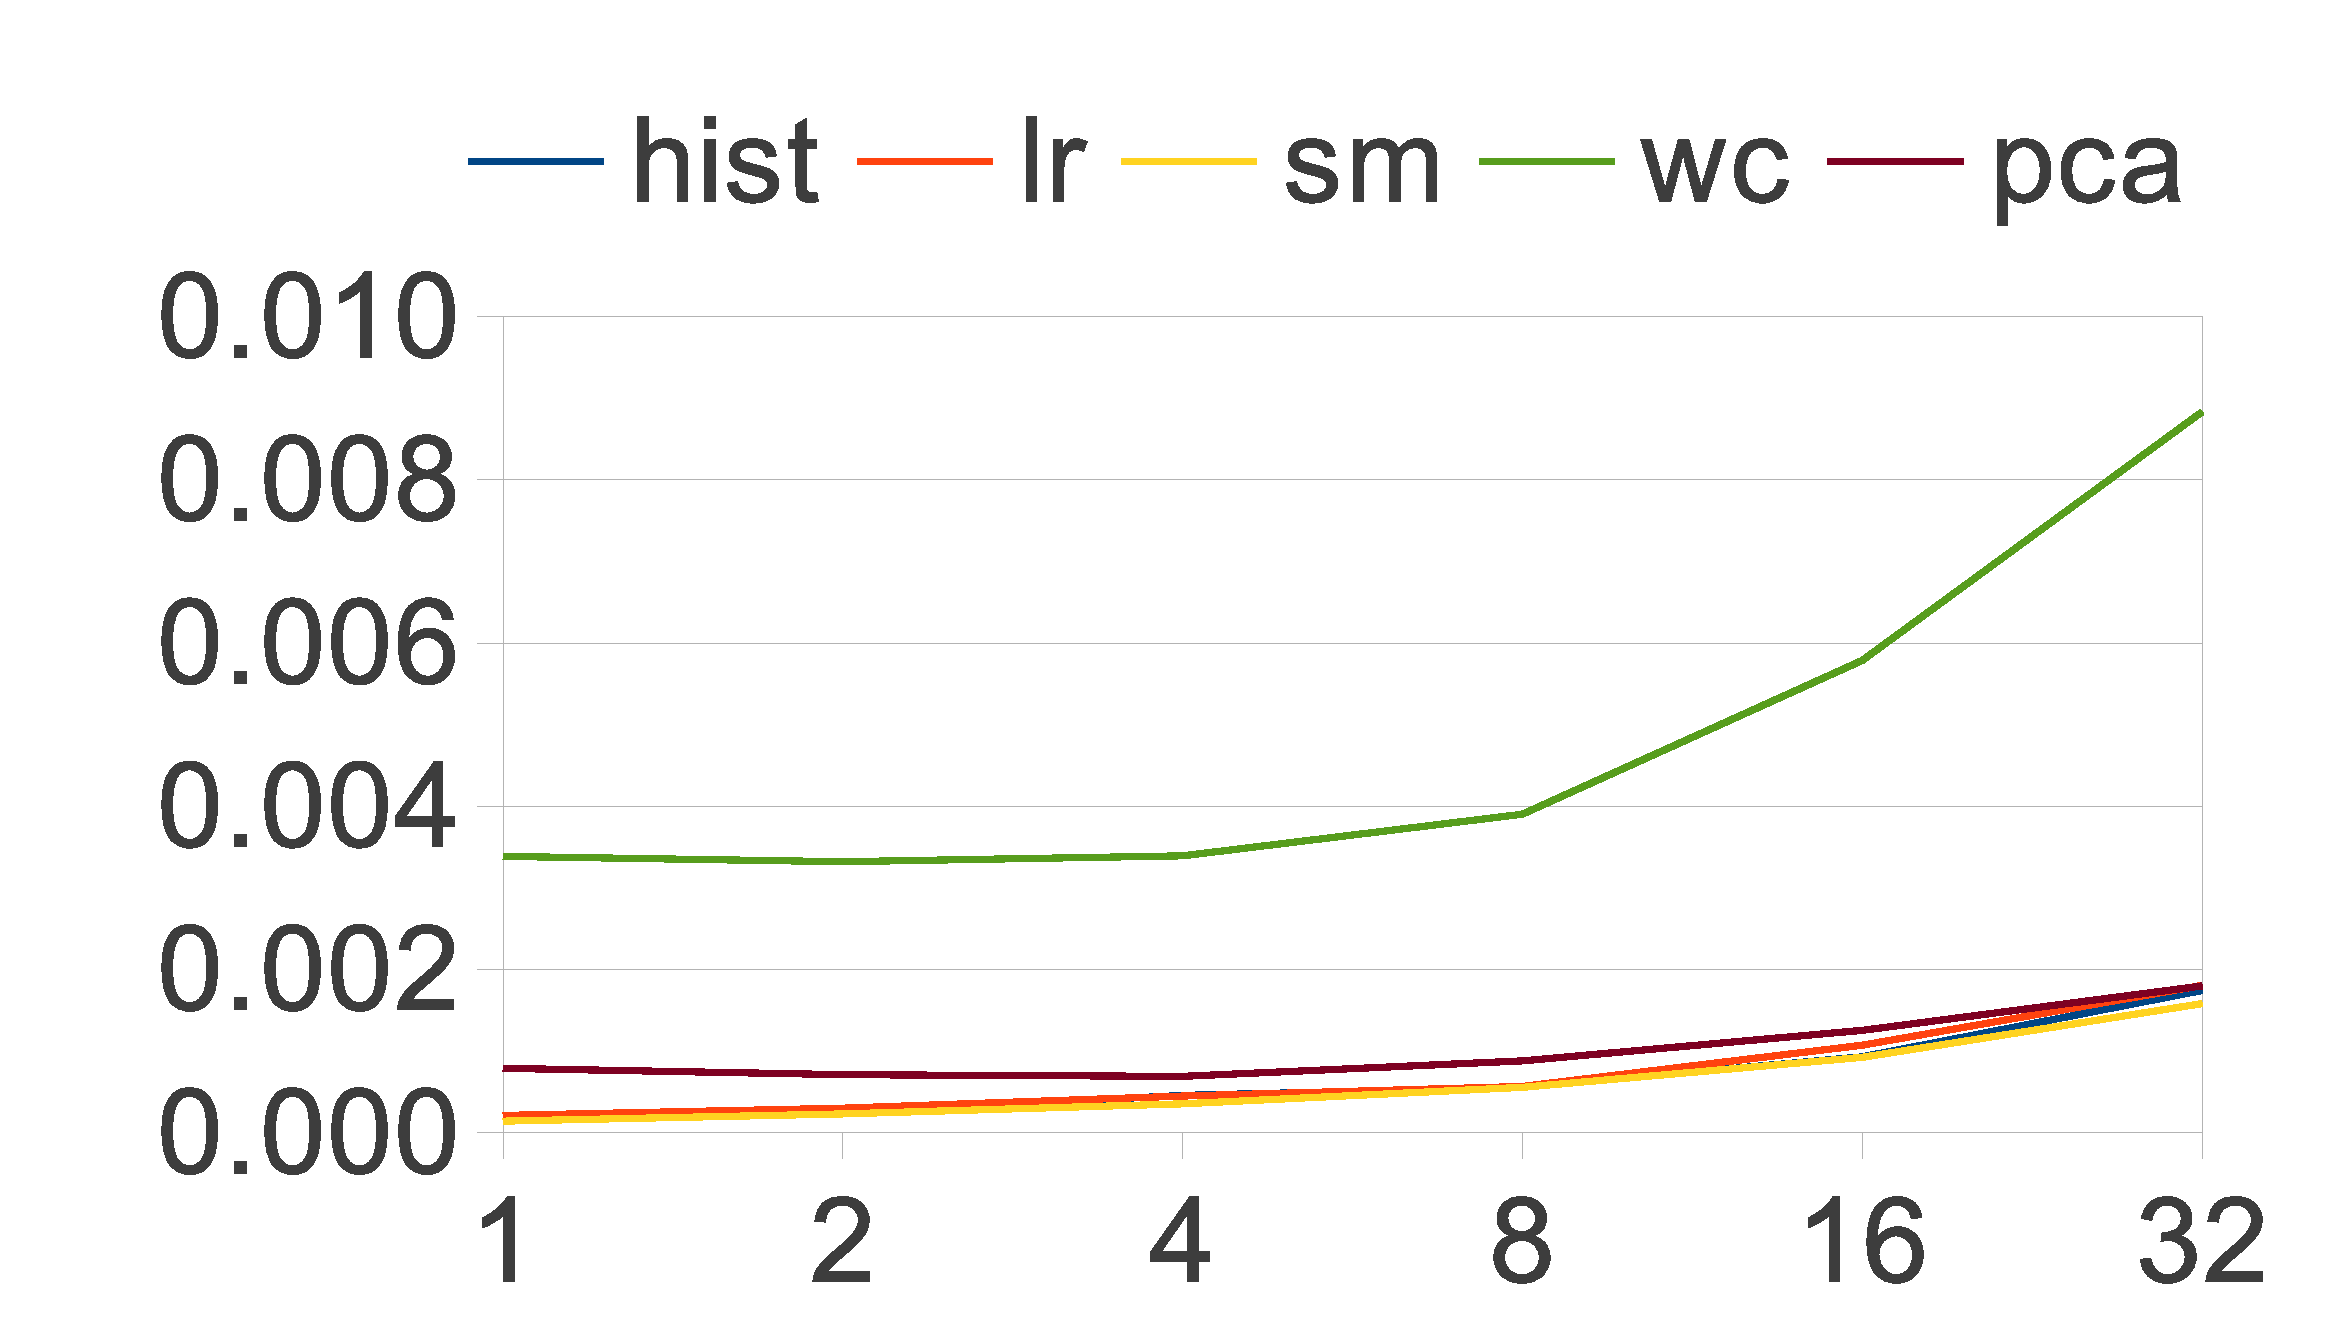
\includegraphics[width=0.25\textwidth]{eps/phoenix_init_time.eps}
   \label{fig:dmr:time:jemalloc}
  }
  \caption{Initialize time of SMR and Phoenix}
   \label{fig:init}
\end{figure}
Figure\ref{fig:init} shows the initialization time of \myds and Phoenix.
The time of \myds used is range 0.25s to  0.35s, 
while it is just about 0.001s in Phoenix.
{\color{red} why the initialization time is so large in \myds}

\begin{figure}[htpb]
\centering
  \subfigure[]{
   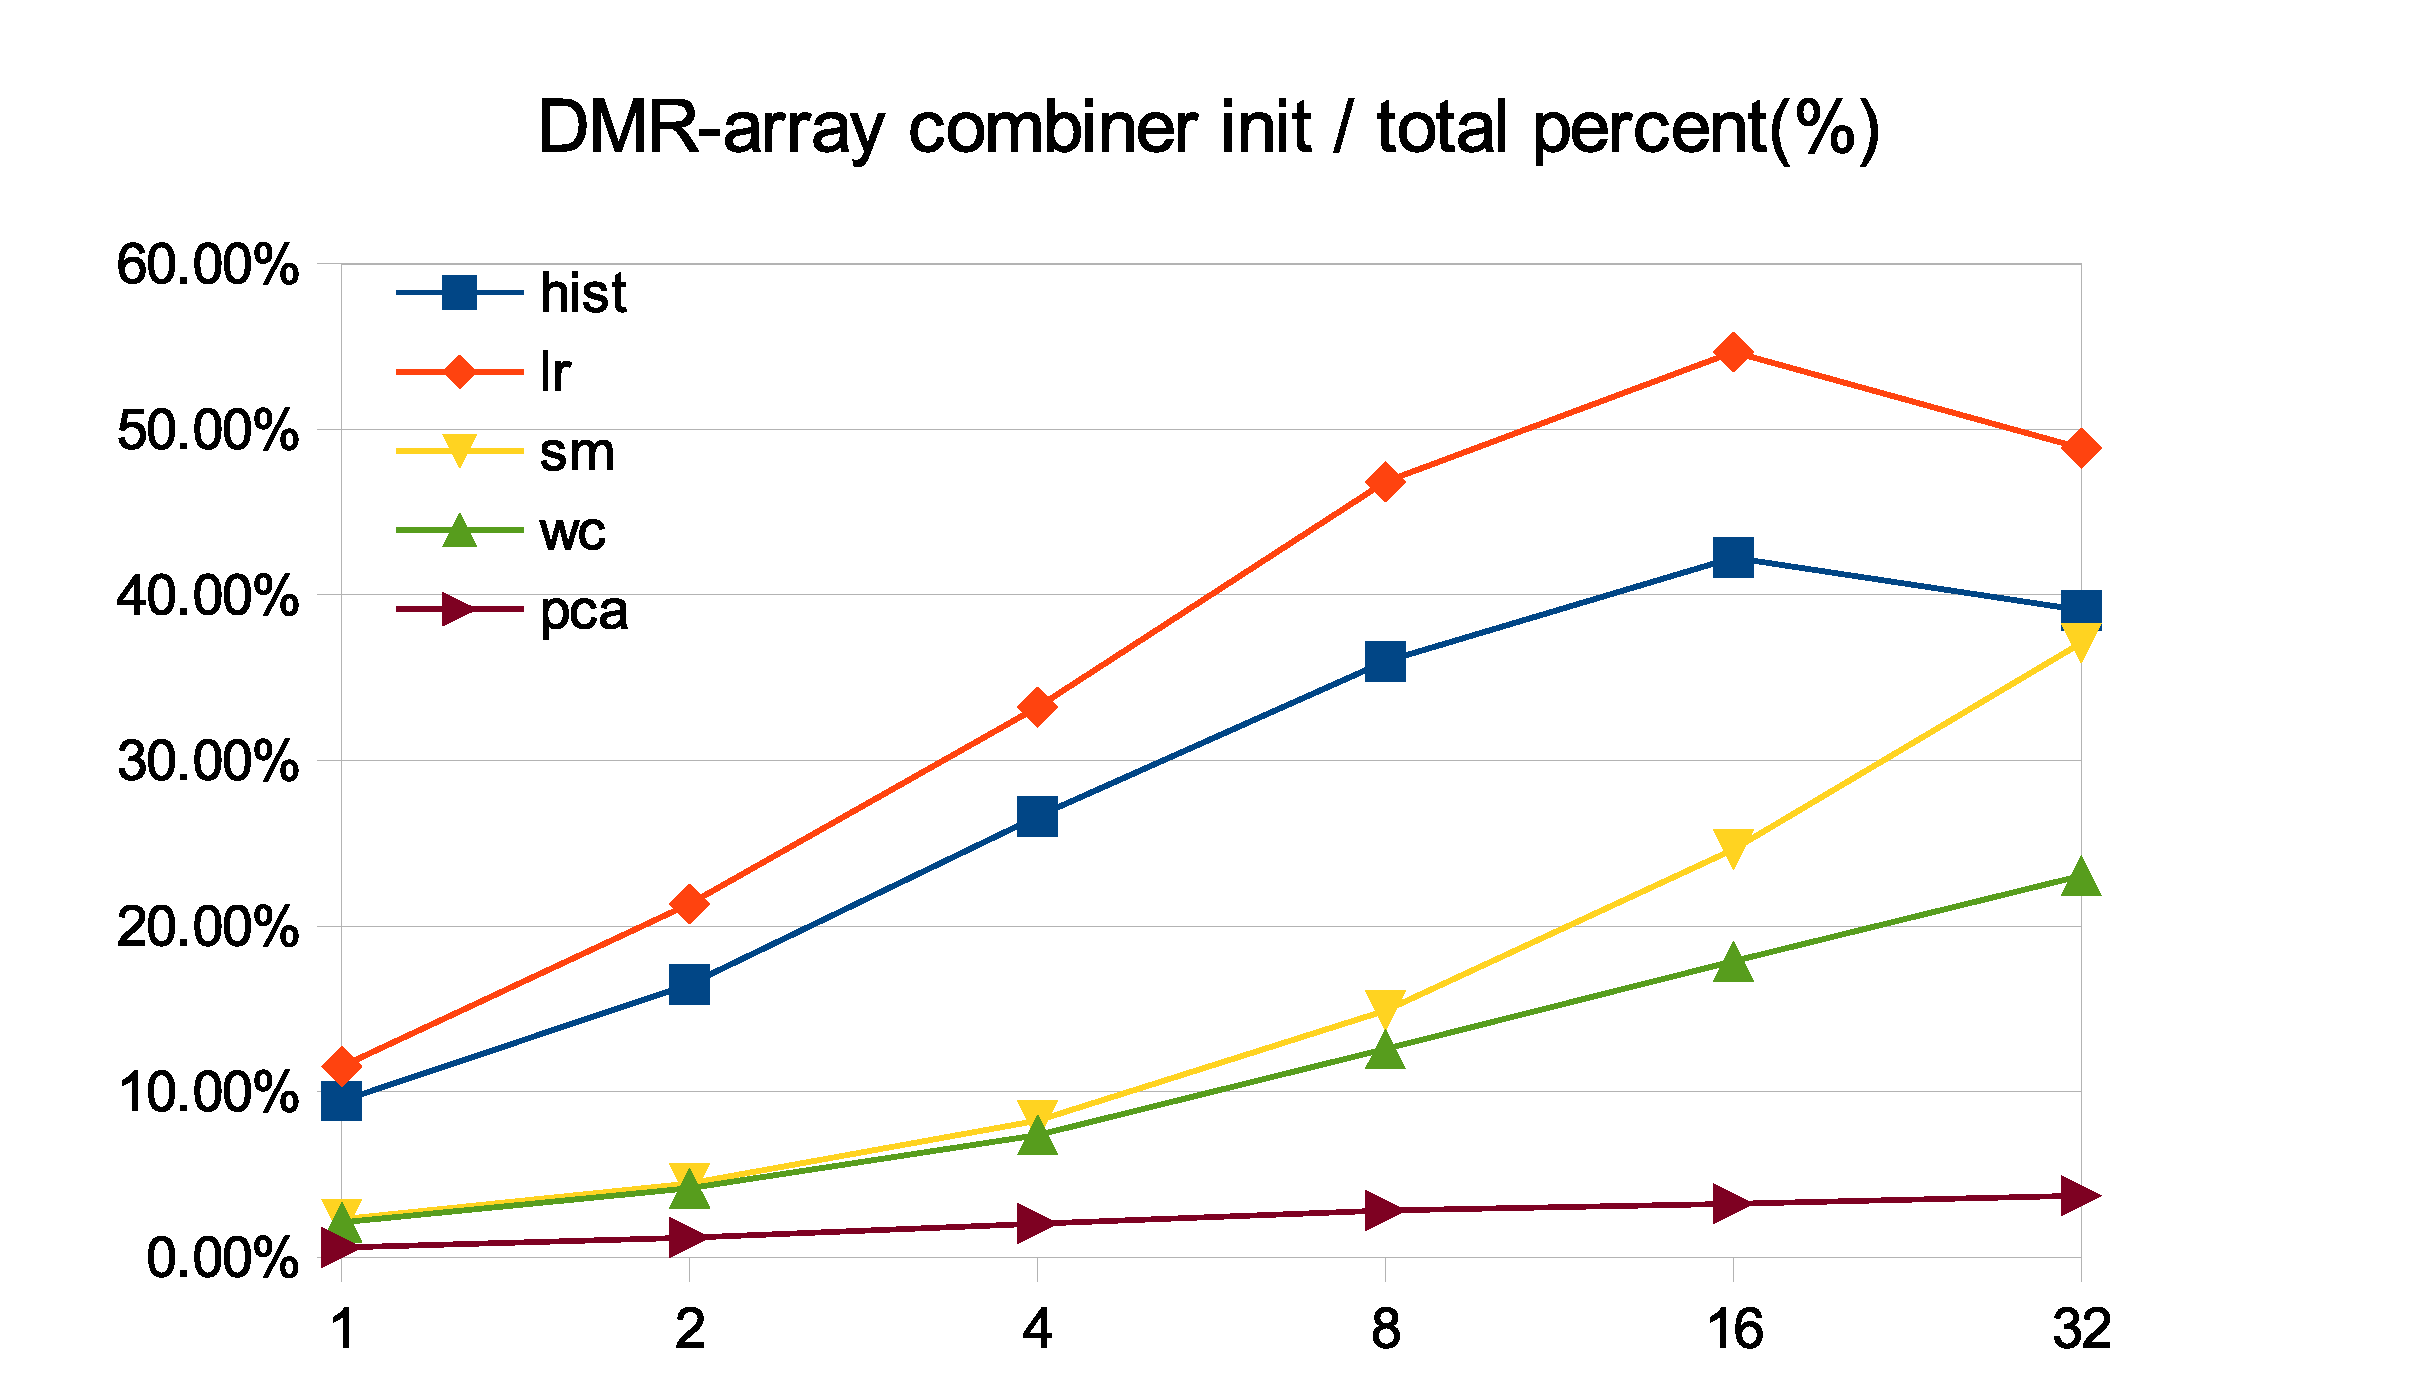
\includegraphics[width=0.4\textwidth]{eps/dmr_init.eps}
   \label{fig:dmr:time:jemalloc}
  }
  \caption{Initialize time of SMR and Phoenix}
   \label{fig:time}
\end{figure}





